\chapter{Introduction}

\section{Overview}
Genetic novelty, a crucial property of all biological systems, originates as mutation. A mutation is the coupling of two components: (1) lesion formation and (2) the subsequent failure of DNA repair systems to recapitulate the original sequence. Through observations of sequence composition alone, it is apparent that the dynamics of this process vary both between species \citep{Karlin1994ComparisonsSequences} and within genomes \citep{Francioli2015Genome-wideHumans}. Although this implies that changes in mutagenesis are a feature of the evolution of DNA sequences, nearly all statistical models in molecular evolution and phylogenetics assume that this property does not exist. 

I refer to the state in which changes to the process of mutation have not yet reached \gls{equilibrium} as mutation disequilibrium. An understanding of the properties of mutagenesis, which includes the existence of mutation disequilibrium, is key to be able to robustly identify when natural selection is operating. Although compositional differences imply historical changes in mutation, they do not guarantee that mutation disequilibrium persists. 

So, how do we know whether mutation disequilibrium exists? Methods that are intended to tackle the existence of mutation disequilibrium have been developed \citep{Squartini2008QuantifyingProcess, Singh2009StrongDrosophila, Ababneh2006Matched-pairsSequences}. Here, I outline the problems with the existing methods and propose new methods for detecting mutation disequilibrium. I demonstrate that the new methods are fit for purpose with a complementary experimental design, coupling simulation studies with analyses of empirical data known to have been subjected to mutation disequilibrium, the process that I am seeking to detect. I focus on evaluating whether the new methods, when applied to such empirical cases, are coherent with the biological basis.

\section{The neutral theory of sequence evolution}

Determining the existence and impact of changes in mutagenesis is required to robustly reject the null and therefore identify when natural selection is operating. The neutral theory of molecular evolution provides a useful null hypothesis for evolution as it proposes that most genetic variation has been affected solely by genetic drift and chance mutation events \citep{Kimura1968EvolutionaryLevel, King1969Non-DarwinianEvolution}. Accordingly, our understanding of the null is dependent on our understanding of the full scope neutral mutagenic processes. 

Measures of sequence composition indicate that the mutagenic process varies significantly between species. Considering, on a chemical level, DNA is the same for very nearly all species, sequence composition can be used as an indirect measure of the processes acting upon a genome \citep{Karlin1994ComparisonsSequences, Karlin1995DinucleotideSignature}. The abundance of nucleotides in a DNA sequence is the `end-product' of the evolutionary process, which is both mutation and natural selection. For strictly neutral sequences, looking at composition is indirectly looking at mutagenesis. Distinct compositions span the tree of life; for example, the percent of nucleotide bases which are either guanine or cytosine (GC content) in \textit{Plasmodium falciparum} is 24\% while \textit{Mycobacterium tuberculosis} is  66\% \citep{Nakamura2000Codon2000}. Such a difference is unlikely to be driven by the composition of functional sequences alone, implying changes in mutagenesis between the two species. 

\section{Global (genome-wide) changes to mutagenesis}

The existence of species-specific mechanisms of lesion formation \citep{Moore2012DNAFunction} and DNA repair \citep{Kelner1949EffectInjury} imply historic mutation disequilibrium on a global genomic scale. Mechanisms of lesion formation (e.g., DNA methylase) and repair (e.g., DNA repair proteins) are encoded within the genome and as a consequence, are subject to forces of evolution \citep{Lynch2010EvolutionRate, Lynch2016GeneticRate}. One example of this is the loss of multiple genes associated with DNA repair in a group of budding yeasts \citep{Steenwyk2019ExtensiveYeasts}. This loss was shown to be accompanied by an increase in mutational load, change in the composition of mutations, and an increase in the rate of evolution \citep{Steenwyk2019ExtensiveYeasts}. A genetic change that modifies either the rate or composition of mutagenesis is defined as a mutator (or antimutator) \citep{Lynch2016GeneticRate}. 

The reported recent loss of the hypermutable base 5-Methylcytosine (hereafter $^5$mC) in \textit{Drosophila melanogaster} is an example of evolution of a global antimutator. 
$^5$mC strongly affects the mutational profile of a species, and accordingly the deletion of the genetic sequence that encodes it is an example of a global evolution of an antimutator. In comparison to non-methylated cytosine, $^5$mC is hypermutable, with higher rates of deamination to thymine \citep{Coulondre1978MolecularColi}. DNA methylation predominantly occurs on cytosines that precede a guanine nucleotide, known as CpG dinucleotides \citep{Holliday1975DNADevelopment}. CpG methylation has been identified in the genomes of a diverse range of invertebrates, including insects \citep{Wang2010EstimatingLoci}. However, the current evidence supports only trace levels of $^5$mC in \textit{D. melanogaster} \citep{Capuano2014CytosineSpecies, Deshmukh2018LevelsGenome}. Critically, the methyltransferases DNMT1 and DNMT3, reported to be necessary for a functional methylation system are not present in the \textit{D. melanogaster} genome, which possesses a sole DNMT2 methyltransferase \citep{Goll2005EukaryoticMethyltransferases, Tweedie1999VestigesMelanogaster}. The level of methylation in \textit{D. melanogaster} is substantially reduced compared to closely related \textit{Drosophila} species, in fact, it is approximately 50 times lower than that in its sister taxa, \textit{Drosophila simulans} \citep{Deshmukh2018LevelsGenome}. These observations suggest that the loss of $^5$mC in \textit{D. melanogaster} occurred after speciation, $\sim 0.8-5.4$ million years ago (MYA) \citep{Cutter2008DivergenceRate, Wang2010EstimatingLoci, Tamura2004TemporalClocks}. This leads to the prediction that the \textit{D. melanogaster} genome, having experienced a recent evolution of a mutator, would globally have a higher level of mutation disequilibrium than \textit{D. simulans}. 

\section{Localised (within-genome) changes to mutagenesis}

Evolvable differences in mutagenesis within a genome demonstrate that the evolution of mutators must also be considered on a local scale. The genome exhibits heterogeneous composition, with substantial changes between regions in terms of GC content \citep{Bernardi1989TheGenome, Bernardi2000IsochoresVertebrates}. A high rate of recombination has been associated with a high rate of mutation to create GC base pairs, implicating recombination as a determinant of observed compositional difference within the genome \citep{Montoya-Burgos2003RecombinationGenomes, Duret2006AEvolution}. Recombination rates are both evolvable and have been shown to differ between human populations \citep{Wegmann2011RecombinationInference}, illustrating a local and evolvable mechanism of lesion formation. Transcription-coupled repair is a mechanism in which the transcribed strand of DNA receives more scrutiny from lesion repair processes \citep{Touchon2003Transcription-coupledGenome}. The transcription of genes is an evolvable property, making transcription-coupled repair a local and evolvable DNA repair phenomenon. 

The \textit{Fxy} gene in \textit{Mus musculus} is an example of a DNA sequence subject to a local change in mutagenesis. In \textit{M. musculus}, \textit{Fxy}, a transcribed gene, spans the boundary of the \gls{Pseudo-Autosomal Region} (PAR) \citep{Palmer1997AMice} (Figure \ref{fig:Fxy}). The PAR is a region of homology between the X and Y chromosomes in mammals, undergoing one obligatory crossover per generation. \textit{Fxy} is X-specific in other \textit{Mus} species, suggesting translocation to the PAR in \textit{M. musculus} after divergence with \textit{Mus spretus}, between 2-3MYA \citep{Huang2005HowMammals}. The boundary to the PAR falls within intron 3 of \textit{Fxy} \citep{Palmer1997AMice}. The half of \textit{Fxy} located in the PAR where there is frequent recombination exhibits differing rates of evolution to the strictly X-specific half where there is little recombination \citep{Perry1999EvolutionaryPosition}. \textit{Fxy} is thus an interesting natural experiment involving a genomic sequence putatively subject to a new mutagenic environment. There is a strong expectation that there would be a local elevation of mutation disequilibrium within the gene, in the PAR-located half because of its new environment. 

\begin{figure}[htbp]
\centering
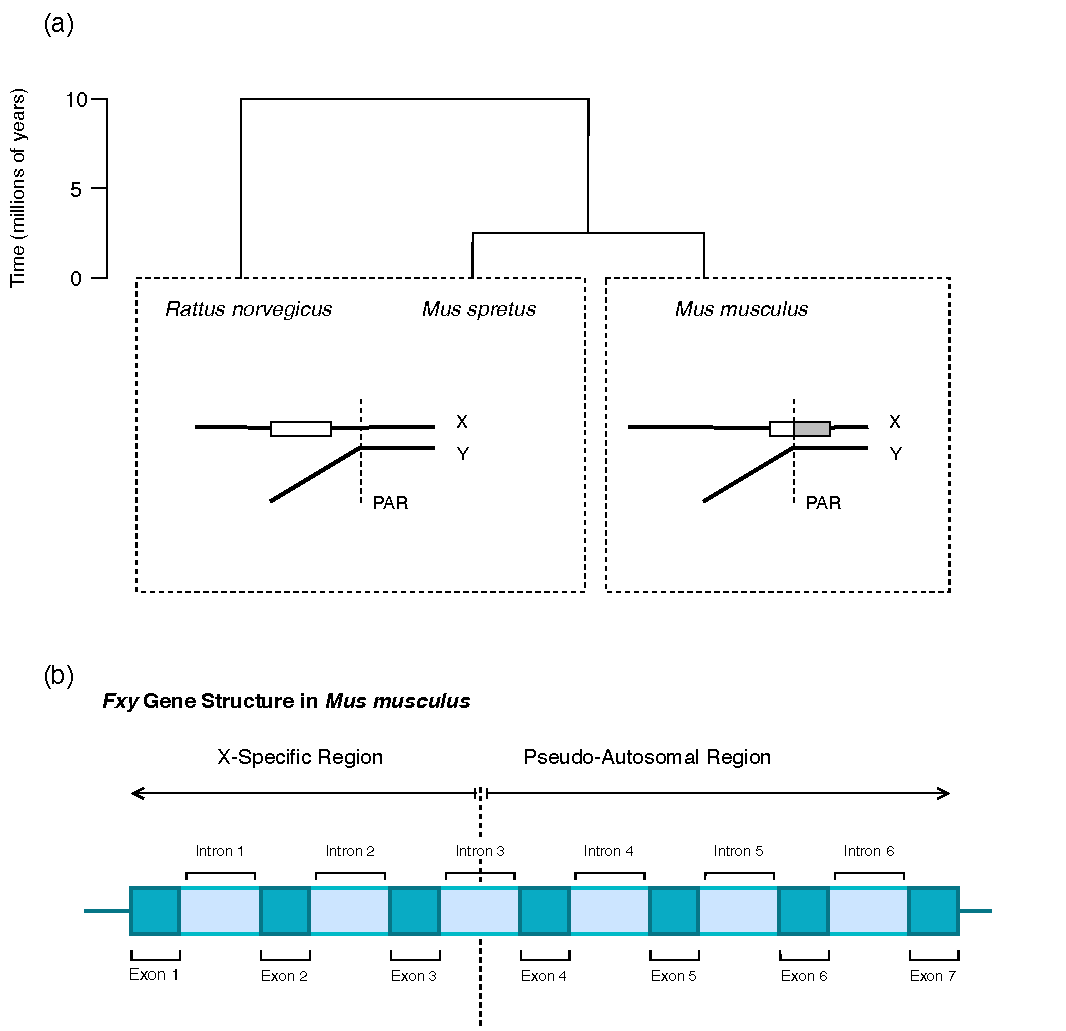
\includegraphics[width=\textwidth]{figures/diagrams/Fxy.pdf}
\caption[Evolutionary History of \textit{Fxy} in Rodents]{\textbf{Evolutionary History of \textit{Fxy} in Rodents}. \textbf{(a)} The \textit{Fxy} gene in \textit{M. musculus} was translocated from a X-specific position to a new position in which it overlaps with the PAR. The overlap in \textit{M. musculus} is shown as the shaded region of the gene, shown as a box. The divergence timescale is indicated in millions of years. In rodents and other mammals \textit{Fxy} is X-specific, suggesting translocation to the PAR in \textit{M. musculus} after divergence with \textit{M. spretus}, between 2-3 million years ago \citep[adapted from Figure 1][]{Galtier2007AdaptationEvolution}. \textbf{(b)} The structure of the \textit{Fxy} gene in \textit{M. musculus}. The $5'$ end of the gene, exons 1-3, are X-specific. The $3'$ end of the gene, exons 4-10, are positioned in the PAR. Note that for simplicity, exons beyond exon 7 are not shown in the structure. The boundary to the PAR falls in intron 3 of \textit{Fxy} \citep{Palmer1997AMice}. }
\label{fig:Fxy}
\end{figure}

The relative levels of purifying natural selection operating on a genomic segment allow for predictions of the magnitude of mutation disequilibrium. The abundance of functional elements in the genome outside of protein coding sequence (CDS) is very low \citep{Graur2013OnENCODE}. Accordingly, changes in intronic sequences are unlikely to be detrimental, making introns a useful neutral benchmark, or at least likely to be subject to a higher rate of mutation \citep{Graur2013OnENCODE}. Consequently, I expect CDS to exhibit a higher magnitude of mutation disequilibrium than intronic sequences that it flanks. For hetero-gametic sexes, you expect the chromosome that is hemizygous to be subjected to more stringent natural selection, because recessive deleterious alleles are exposed in the hemi-zygous sex \citep{Charlesworth1987TheAutosomes}. Given existing mutation disequilibrium, it is probable that an increased magnitude of purifying selection should slow the rate of convergence to equilibrium, and thus lead to a higher magnitude of disequilibrium. Accordingly, X-chromosome sequences should exhibit a higher magnitude of disequilibrium relative to autosomal sequences. 

Testing for mutation disequilibrium requires appropriate \gls{models} of sequence divergence. \Gls{Substitution models} impose varying assumptions on the divergence process, including, but not limited to: reversibility, that the process is identical to how it would appear if run in reverse; and \gls{stationarity}, the process is in \gls{equilibrium}. The evidence indicates the occurrence of, at the very least, historical changes in mutagenesis, in turn implying periods of mutation disequilibrium have existed in the past. However, this observation does not guarantee that disequilibrium persists. In order to interrogate this, I need models which are appropriate and fit for purpose. This is a non-reversible and non-stationary model for the alternate hypotheses (the existence of mutation disequilibrium), and a non-reversible but stationary model for the null (no mutation disequilibrium). 

\section{Previous work in detecting mutation disequilibrium}

Methods that are intended to tackle the statistical problem of testing for mutation disequilibrium have been proposed before, but not without limitations. \cite{Ababneh2006Matched-pairsSequences} introduced matched-pairs tests of homogeneity, looking at the internal and marginal symmetry of the nucleotide composition. These methods, however, are limited in power because they operate on pairs of sequences. To test for the existence of disequilibrium \cite{Squartini2008QuantifyingProcess} use a $\chi^2$-test comparing the current and equilibrium nucleotide distributions. The test proposed by \cite{Squartini2008QuantifyingProcess} appears to have a good theoretical basis, however, they do not evaluate whether the test statistic is consistent with the asymptotic approximations, or demonstrate that it behaves in a reliable manner. It remains unclear as to whether the methods are, in fact, reasonable. 

Methods of quantifying mutation disequilibrium have been developed, but do not measure all possible changes. \cite{Singh2009StrongDrosophila} introduced a time to equilibrium calculation of the GC content of a single \gls{edge} using a non-stationary but strand-symmetric process. \cite{Squartini2008QuantifyingProcess} introduced a method of quantifying disequilibrium using three indices, calculated from differences in the current and equilibrium nucleotide composition. Although defined for a general process, their work is demonstrated solely with a strand-symmetric model. Thus, both methods only consider changes in terms of GC content and consequently do not capture the complete scope of possible changes.

The detailed metadata now associated with genomes creates a wealth of new opportunities for methods development, enabling the inclusion of data of natural origins in experimental design. Traditional approaches to methods development relied near entirely on simulation studies for establishing the properties of a new method, and that is no longer adequate. The comprehensive understanding of the genetic underpinnings of methylation is what has provided the confidence of declaring that \textit{D. melanogaster} has recently lost this major mutagenic component in its genome. Therefore, it is a lineage that constitutes a positive control for the methods I seek to develop, and its sister taxa constitutes a relative negative control. The characterisation of the PAR in \textit{M. musculus} has allowed for the conjectured impact of translocation of the \textit{Fxy} gene. \textit{Fxy} provides another empirical control, the PAR located half is a positive control and the strictly X-linked half is the relative negative control. In addition to demonstrating consistency with asymptotic approximations and capturing the full scope of changes, these empirical controls are an essential extension of my methods relative to work previously done in the field. 

\section{Aims and scope}

In this work, I tackle the statistical problem of identifying the existence of mutation disequilibrium, its magnitude and whether it is equivalent between samples. Employing a complementary experimental design to interrogate natural occurrences of mutation disequilibrium on proposed positive controls, I address the following questions. Firstly, is there more mutation disequilibrium and does it have a greater magnitude in \textit{D. melanogaster} than in \textit{D. simulans}? Similarly, is this true for the PAR located component of \textit{Fxy} compared to the X-specific component in \textit{M. musculus}? Finally, I evaluate whether our own genome is in equilibrium. 

The results from the positive controls were striking in their consistency with the predictions. Consistent with the expectations of the neutral theory, genomic regions subjected to purifying natural selection are associated with higher incidence and magnitude of mutation disequilibrium. Results from the analysis of our genome indicate that the majority of our genome is not at equilibrium. I then discuss the implication of these results on our understanding of mutagenesis and future methods development in molecular biology. 